\section{Modelo de Efectos Fijos}

\begin{figure}[t]
\centering
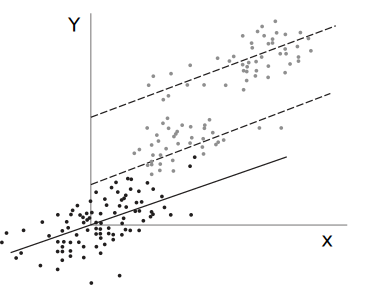
\includegraphics[scale=1]{images/fixed_effects_example.pdf}
\caption{Ejemplo de efectos fijos}
\label{fig:efectos_fijo}
\end{figure}



\newcommand{\slopeestim}[1] { $\estslope \sim #1$ }

El modelo agrupado o pooled que vimos en el anterior capítulo posee un problema, ya que niega la posibilidad de heterogeneidad no observada, que son variables no medidas que afectan al sistema. En el caso concreto de nuestro corpus, dicha heterogeneidad puede deberse a multiplicidad de factores no medidos en él, como por ejemplo: la personalidad de los sujetos es un factor no medido y que puede influír en la dinámica de la interacción entre estos.

Los modelos de efectos fijos nos ayudan a controlar la heterogeneidad no observada cuando ésta es constante en el tiempo.
Como el entrainment que medimos mediante el proceso TAMA es un proceso direccional (es decir, medimos tanto la influencia de un interlocutor sobre el otro y viceversa), definimos los ``grupos'' como las observaciones de entrainment y sus variables sociales de una sesión y el interlocutor sobre el cual consideramos la direccionalidad, tal y cual lo definimos en una sección anterior. esto nos arroja la cantidad de 24 grupos de observaciones



\section{Definición Formal de Efectos Fijos}

NOTA: Escribir esto

\section{Resultados}

Utilizando como variable explicativa el \entrainment, los resultados no son son significativos. En (NOTA: agregar referencia a las tablas) podemos observar la tabla de coeficientes de esta regresión de efectos fijos.

Por otro lado, este modelo utilizando como variable independiente al valor absoluto del \entrainment dio valores sustancialmente apreciables. Las variables a/p \ENGMAX, \FOMEAN y \NOISETOHARMONICS poseen valores altamente significativos ( p-valor menor a 0.05) para al menos 2 variables sociales. En la tabla \ref{regresion_efectos_fijos_tabla} podemos ver la tabla del test de coeficientes con las variables sociales significativas resaltadas. Una versión simplificada tabla la podemos ver en \ref{sign_table} que grafica mediante tabla de doble entrada aquellos pares de variables a/p y variables sociales con coeficientes significativos y su signo.

Con respecto a las variables sociales, podemos observar que:

\begin{itemize}
  \item \svcontributes se relaciona positivamente con el \absentrainment cuando la variable a/p medida es \FOMEAN o bien \NOISETOHARMONICS. Esto significa que, cuando sube el valor absoluto del \entrainment, esta variable positiva también lo hace con buena probabilidad. Esto es un efecto esperable: cuando hay mimetización, hay colaboración para el éxito en el juego.
  \item \svclear, otra variable que refleja una visión positiva del juego, también se relaciona positivamente con el \absentrainment para las variables \FOMEAN, \NOISETOHARMONICS, \ENGMAX como a su vez para \PHONAVG y para \SYLCOUNT
  \item \svengaged, de la misma manera que las dos anteriores, relaciona positivamente pero sólo con \FOMEAN
  \item \svplanning y \svencourages, otras variables positivas, no presentan valores significativos.
  \item \svdifficult, una variable que representa una característica negativa de la conversación, se relaciona de igual con el \absentrainment cuando la variable acústico prosódica es \ENGMAX. esto contiene sentido, ya que a mayor mimetización de los interlocutores, la dificultad de estos para hablar debería disminuir.
  \item La variable \svbored se comporta de idéntica manera, sólo que con \FOMEAN.
  \item \svdislikes no presenta valores significativos
\end{itemize}


\begin{tabular}{rrrrr}
  \hline
 \ENGMAX & Estimate & Std. Error & t value & Pr($>$$|$t$|$) \\
  \hline
contributes\_to\_successful\_completion & 0.0497 & 0.4262 & 0.1165 & 0.9074 \\
  \myhighlight making\_self\_clear & 1.6581 & 0.3864 & 4.2909 & 0.0001 \\
  engaged\_in\_game & 0.3307 & 0.2576 & 1.2840 & 0.2008 \\
  planning\_what\_to\_say & 0.5005 & 0.5327 & 0.9395 & 0.3487 \\
  gives\_encouragement & 0.4264 & 0.3792 & 1.1246 & 0.2622 \\
  \myhighlight difficult\_for\_partner\_to\_speak & -0.7200 & 0.2858 & -2.5190 & 0.0126 \\
  bored\_with\_game & 0.2163 & 0.2560 & 0.8450 & 0.3992 \\
  dislikes\_partner & -0.4318 & 0.3443 & -1.2541 & 0.2114 \\
   \hline
\end{tabular}

\begin{tabular}{rrrrr}
  \hline
 \FOMEAN & Estimate & Std. Error & t value & Pr($>$$|$t$|$) \\
  \hline
 \myhighlight contributes\_to\_successful\_completion & 1.0274 & 0.3025 & 3.3962 & 0.0008 \\
  \myhighlight making\_self\_clear & 0.8307 & 0.3934 & 2.1115 & 0.0361 \\
  \myhighlight engaged\_in\_game & 0.8850 & 0.2750 & 3.2182 & 0.0015 \\
  planning\_what\_to\_say & 0.7167 & 0.5400 & 1.3273 & 0.1860 \\
  gives\_encouragement & 0.0075 & 0.3941 & 0.0190 & 0.9848 \\
  difficult\_for\_partner\_to\_speak & -0.5975 & 0.3928 & -1.5209 & 0.1300 \\
  \myhighlight bored\_with\_game & -0.7586 & 0.2481 & -3.0572 & 0.0026 \\
  dislikes\_partner & 0.0371 & 0.3800 & 0.0977 & 0.9223 \\
   \hline
\end{tabular}

\begin{tabular}{rrrrr}
  \hline
 \NOISETOHARMONICS & Estimate & Std. Error & t value & Pr($>$$|$t$|$) \\
  \hline
\myhighlight contributes\_to\_successful\_completion & 0.7041 & 0.3404 & 2.0686 & 0.0400 \\
  \myhighlight making\_self\_clear & 1.3344 & 0.3537 & 3.7725 & 0.0002 \\
  engaged\_in\_game & 0.0954 & 0.3462 & 0.2756 & 0.7832 \\
  planning\_what\_to\_say & -0.1874 & 0.4177 & -0.4485 & 0.6543 \\
  gives\_encouragement & 0.7234 & 0.4782 & 1.5127 & 0.1321 \\
  difficult\_for\_partner\_to\_speak & -0.1941 & 0.3436 & -0.5648 & 0.5729 \\
  \myhighlight bored\_with\_game & 0.5876 & 0.3028 & 1.9404 & 0.0539 \\
  dislikes\_partner & 0.3582 & 0.3330 & 1.0755 & 0.2835 \\
   \hline
\end{tabular}

\begin{figure}[ht]
\centering
% psl is "Positive Slope"
\newcommand{\psl} { $+$ }
\newcommand{\ppsl} { $++$ }
\newcommand{\pppsl} { $+++$ }

% nsl stands for "Negative SLope"
\newcommand{\nsl} { $-$ }
\newcommand{\nnsl} { $--$ }
\newcommand{\nsl} { $---$ }


\begin{tabular}{| c | c | c | c | c | c |}
  \hline
               &\ENGMAX  & \ENGMEAN  & \FOMEAN  & \FOMAX  & NOISERATIO  \\
  \hline
  contributes  &         &           & \psl     &         & \psl        \\ \hline
  clear        & \pppsl  &           & \psl     &         & \psl        \\ \hline
  engaged      &         &           & \psl     &         &             \\ \hline
  planning     &         &           &          &         &             \\ \hline
  encourages   &         &           &          &         &             \\ \hline
  difficult    & \nsl    &           &          &         &             \\ \hline
  bored        &         &           & \nsl     &         &             \\ \hline
  dislikes     &         &           &          &         &             \\ \hline
  \hline
& PHON\_AVG & PHON\_COUNT & SHIMMER & SYL\_AVG & SYL\_COUNT \\
  \hline
contributes  &      &  &  &  &        \\ \hline
  clear      & \psl &  &  &  & \psl   \\ \hline
  engaged    &      &  &  &  &        \\ \hline
  planning   &      &  &  &  &        \\ \hline
  encourages &      &  &  &  &        \\ \hline
  difficult  &      &  &  &  &        \\ \hline
  bored      &      &  &  &  &        \\ \hline
  dislikes   &      &  &  &  &        \\ \hline
  \hline
\end{tabular}


\caption{Tabla que representa los resultados significantes del experimento. En una de las entradas, tenemos los nombres abreviados de las variables sociales, y en la otra las variables a/p. El símbolo \psl representa valor significante y positivo de la pendiente de la regresión de efectos fijos, mientras que \nsl representa significante y negativo }

\label{sign_table}

\end{figure}

